\section{Utilizzo di Butterfly}\label{utilizzo}

\subsection{Gestore Personale}

Il Gestore Personale è la componente principale di \progetto\ e si può suddividere in due sotto-componenti:

\begin{itemize}
    \item Interfaccia utente
    \item Message processor, che contiene la logica di business di \progetto
\end{itemize}

Il secondo non è di pertinenza di questo manuale (ma del \MSd), in quanto l'utente non lo utilizza direttamente, per cui verrà solamente discusso l'utilizzo del sistema tramite l'interfaccia utente.

\subsubsection{Autenticazione}
È possibile effettuare l'autenticazione all'interno del sistema tramite il link del container sul quale è in esecuzione, specificato nella configurazione effettuata precedentemente.
Per effettuare correttamente l'autenticazione è necessario l'inserimento del proprio ID Telegram o Email con il quale si è iscritti nel sistema.
\begin{figure}[H]
	\centering
	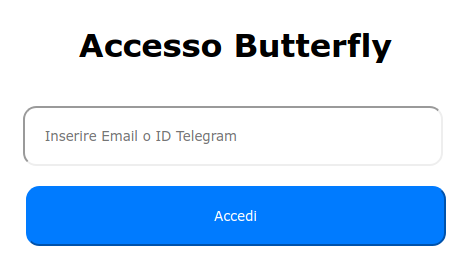
\includegraphics[width=10cm]{img/accesso_1.png}
	\caption{Form di accesso al sistema}
\end{figure}
In caso l'identificativo inserito non fosse valido, e non corrispondesse quindi a un match nel database, verrà mostrato all'utente un messaggio di errore.
\begin{figure}[H]
	\centering
	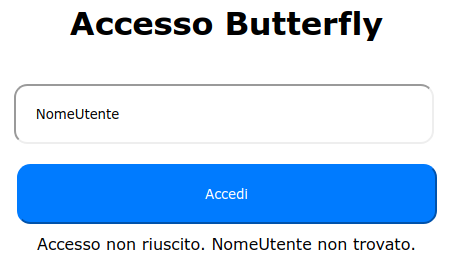
\includegraphics[width=10cm]{img/accesso_2.png}
	\caption{Messaggio di errore durante accesso al sistema}
\end{figure}
Nel caso in cui un utente non autenticato cerchi di accedere ad una sezione per cui non ha i privilegi, questo verrà rimandato alla pagina di autenticazione.\par
Se un utente iscritto correttamente nel sistema ha inserito sia indirizzo Email che ID Telegram, allora può accedere utilizzando indipendentemente il primo o il secondo.

\subsubsection{Pannello di controllo}
Dopo aver effettuato l'accesso al sistema, si viene rimandati alla pagina relativa al Pannello di controllo che contiene i comandi principali per la navigazione del sito e le operazioni che un utente può eseguire.
Le sezioni a cui si può navigare dal Pannello di controllo sono:
\begin{itemize}
	\item inserimento di un nuovo utente
	\item rimozione di un utente
	\item modifica dei propri dati
	\item modifica delle proprie preferenze
\end{itemize}
\begin{figure}[H]
	\centering
	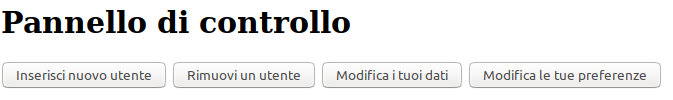
\includegraphics[width=14cm]{img/pannello_1.png}
	\caption{Interfaccia modifica preferenze}
\end{figure}

\subsubsection{Iscrizione a Butterfly}
L'iscrizione al sistema \progetto\ è permessa, secondo i requisiti del capitolato, solamente tramite l'utilizzo delle API Rest (come descritto in \S\ref{APIRest}) oppure è permesso agli utenti già registrati di inserirne altri.
La sezione di inserimento di un nuovo utente è raggiungibile dal Pannello di controllo e prevede l'inserimento dei seguenti dati:
\begin{itemize}
	\item Nome
	\item Cognome
	\item Email
	\item Telegram
\end{itemize}
È necessario inserire almeno un campo a scelta tra Email e Telegram.
Nel caso questi fossero già associati ad un utente iscritto a \progetto\ verrà visualizzato un messaggio di errore.
\begin{figure}[H]
	\centering
	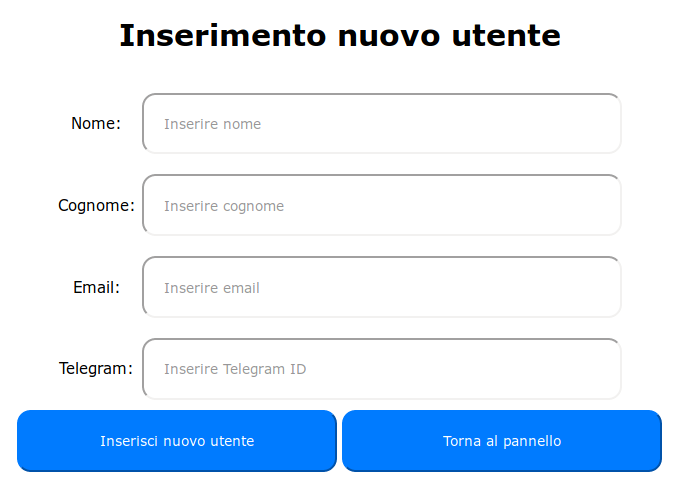
\includegraphics[width=\textwidth]{img/inserimento_1.png}
	\caption{Interfaccia inserimento nuovo utente}
\end{figure}

\subsubsection{Modifica preferenze}\label{preferenze}
La modifica delle preferenze è possibile solamente per utenti già iscritti ed autenticati nel sistema.
È raggiungibile tramite il Pannello di Controllo sotto la voce ``Modifica le tue preferenze''.
In questa sezione si possono trovare le principali impostazioni del sistema dal punto di vista dell'utente finale:
\begin{itemize}
	\item Lista dei progetti a cui si è iscritti
	\item Modifica della priorità assegnata ad un progetto
	\item Lista dei Topic (formati dall'insieme di Label e Keyword) disponibili e iscrizione o disiscrizione da questi, che vengono mostrati dinamicamente in base ai progetti a cui si è iscritti.
	\item Inserimento dei giorni di indisponibilità
	\item Impostare su quale delle due piattaforme (Email o Telegram) ricevere le notifiche
\end{itemize}
Le Label non sono modificabili in quanto vengono aggiornate solamente da una componente del Gestore Personale che le memorizza quando avvengono update alle issue relative ai progetti.
Le Keyword, invece, sono formate da una lista di parole che possono essere contenute nei messaggi di push di GitLab e di cui si è interessati a ricevere notifiche.
\begin{figure}[H]
	\centering
	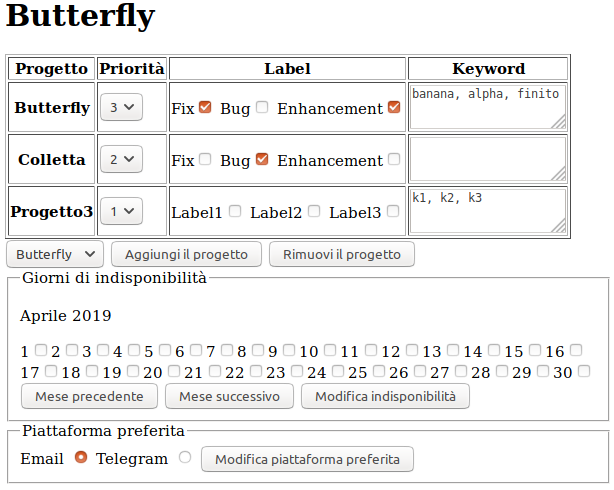
\includegraphics[width=12cm]{img/preferenze_1.png}
	\caption{Interfaccia modifica preferenze}
\end{figure}

\subsubsection{Modifica dei propri dati}
La modifica dei propri dati è possibile attraverso la sezione ``Modifica i tuoi dati'' accessibile dal Pannello di controllo.
Qui un utente può modificare i dati forniti in fase di registrazione.
\begin{figure}[H]
	\centering
	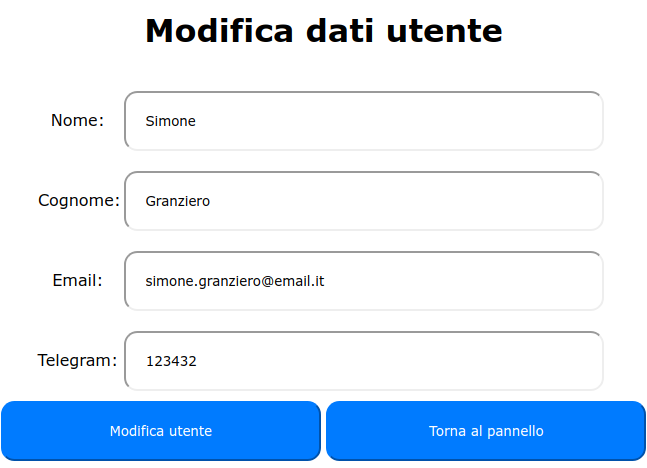
\includegraphics[width=\textwidth]{img/modifica_1.png}
	\caption{Modifica dei dati di un utente}
\end{figure}
Come nella registrazione di un nuovo utente, nel caso questi fossero già associati ad una persona iscritta a \progetto\ verrà visualizzato un messaggio di errore.

\subsubsection{Uscita dal sistema}
Per effettuare il logout dal sistema, cliccare sul bottone ``Logout'' presente in alto a destra di ciascuna pagina.

\subsubsection{Rimozione di un utente dal sistema}
Viene data la possibilità di rimuovere un utente dal sistema eliminando quindi i suoi dati precedentemente salvati nel database.
La rimozione è possibile attraverso la sezione ``Rimuovi un utente'' accessibile dal Pannello di controllo.
\begin{figure}[H]
	\centering
	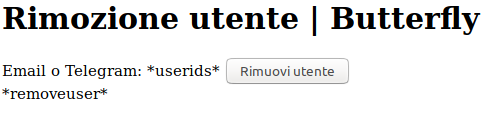
\includegraphics[width=12cm]{img/rimozione_1.png}
	\caption{Interfaccia rimozione di un utente}
\end{figure}
Nel caso in cui un utente desideri eliminare il proprio profilo dal sistema, dopo aver selezionato il proprio identificativo e cliccato il pulsante ``Rimuovi utente'', verrà effettuato il logout automatico.

\subsection{API Rest}\label{APIRest}
\newcommand{\homeUrl}{home\_url}

Per la gestione delle risorse di \progetto\ abbiamo utilizzato lo standard architetturale delle API Rest.
Nelle sezioni successive viene descritto come interagire con le API fornite dal sistema.
Il root path sottinteso sarà sempre \texttt{\homeUrl/api/v1/}.
Ad esempio, per effettuare la GET dell'user \texttt{@user1}, l'indirizzo sarà:
\begin{center}
    \texttt{GET \homeUrl/api/v1/user/@user1}
\end{center}

\subsubsection{User}

\texttt{User} è la risorsa utente.
È possibile visualizzare, aggiungere, modificare o rimuovere gli utenti tramite una semplice
richiesta HTTP.

\paragraph{Visualizzazione}
È possibile visualizzare i dati di un utente tramite la richiesta
    \begin{center}
        \texttt{GET  /user/<id>}
    \end{center}

\paragraph{Inserimento}
È possibile inserire un nuovo utente tramite la richiesta
    \begin{center}
        \texttt{PUT /user}
    \end{center}

È possibile dare i seguenti campi di tipo stringa alla richiesta, per aggiungere in fase di creazione i dati:
\begin{itemize}[noitemsep]
    \item \texttt{name}
    \item \texttt{surname}
    \item \texttt{telegram}
    \item \texttt{email}
\end{itemize}
Almeno uno tra i campi \texttt{email} e \texttt{telegram} vanno fornite insieme al payload.

\paragraph{Modifica}

È possibile modificare un utente tramite la richiesta
\begin{center}
    \texttt{POST /user/<id>}
\end{center}

È possibile dare i seguenti campi di tipo stringa alla richiesta, per aggiungere in fase di creazione i dati:
\begin{itemize}[noitemsep]
    \item \texttt{name}
    \item \texttt{surname}
    \item \texttt{telegram}
    \item \texttt{email}
\end{itemize}


\paragraph{Rimozione}

È possibile rimuovere un utente dal sistema \progetto\ con la richiesta
\begin{center}
    \texttt{DELETE /user/<id>}
\end{center}

Se il campo \texttt{<id>} corrisponde a un ID presente nel sistema, esso verrà rimosso.


\paragraph{Riepilogo}

\begin{table}[H]
    \begin{paddedtablex}[1.3]{\textwidth}{cYY}
        \thead{Metodo HTTP} & \thead{URI} & \thead{Action}\\\toprule
        \texttt{GET} & \texttt{/user/<id>} & Restituisce un payload in JSON dell'utente che corrisponde a \texttt{<id>}\\
        \texttt{PUT} & \texttt{/user} & Inserisce un nuovo utente. È necessario fornire uno tra i campi telegram o email\\
        \texttt{POST} & \texttt{/user/<id>} & Modifica l'utente corrispondente a \texttt{<id>} con i campi passati nella richiesta\\
        \texttt{DELETE} & \texttt{/user/<id>} & Elimina l'utente corrispondente a \texttt{<id>} dal sistema\\
        \bottomrule
    \end{paddedtablex}
    \caption{Riepilogo delle Rest API per la risorsa User}
\end{table}


\subsubsection{Preference}
Preference è la risorsa preferenza. È possibile visualizzare, aggiungere, modificare o rimuovere le preferenze di un utente tramite una semplice richiesta HTTP.

\paragraph{Visualizzazione}
È possibile visualizzare le preferenze di un utente tramite la richiesta
    \begin{center}
        \texttt{GET  /preference/<user>/<id>}
    \end{center}
Se il campo \texttt{<user>} corrisponde a un utente presente nel sistema e il campo \texttt{<id>} corrisponde a un tipo di preferenza, verranno mostrati i dati relativi a tale preferenza.

I tipi di preferenza disponibili sono:
\begin{itemize}[noitemsep]
    \item \texttt{progetto}
    \item \texttt{disponibilità}
    \item \texttt{piattaforma}
\end{itemize}

\paragraph{Inserimento}
È possibile inserire una nuova preferenza tramite la richiesta
    \begin{center}
        \texttt{PUT /preference/<user>/<id>}
    \end{center}

È possibile fornire dei campi di tipo stringa alla richiesta, in base al tipo della risorsa, per aggiungere dati in fase di creazione.
In base al tipo della preferenza, i campi sono:
\begin{itemize}[noitemsep]
    \item progetto
        \begin{itemize}[noitemsep]
            \item \texttt{nome}
            \item \texttt{priorità}
            \item \texttt{labels}
            \item \texttt{keywords}
        \end{itemize}
    \item disponibilità
        \begin{itemize}[noitemsep]
            \item \texttt{data}
        \end{itemize}
    \item piattaforma
        \begin{itemize}[noitemsep]
            \item \texttt{piattaforma}
        \end{itemize}
\end{itemize}


\paragraph{Modifica}

È possibile modificare una preferenza tramite la richiesta
\begin{center}
    \texttt{POST /preference/<user>/<id>}
\end{center}


È possibile fornire dei campi di tipo stringa alla richiesta, in base al tipo della risorsa, per aggiungere dati in fase di creazione.
In base al tipo della preferenza, i campi sono:
\begin{itemize}[noitemsep]
    \item progetto
        \begin{itemize}[noitemsep]
            \item \texttt{nome}
            \item \texttt{priorità}
            \item \texttt{labels}
            \item \texttt{keywords}
        \end{itemize}
    \item disponibilità
        \begin{itemize}[noitemsep]
            \item \texttt{data}
        \end{itemize}
    \item piattaforma
        \begin{itemize}[noitemsep]
            \item \texttt{piattaforma}
        \end{itemize}
\end{itemize}


\paragraph{Rimozione}

È possibile rimuovere una preferenza dal sistema Butterfly con la richiesta
\begin{center}
    \texttt{DELETE /preference/<user>/<id>}
\end{center}

Se il campo \texttt{<user>} corrisponde a un ID presente nel sistema e il campo \texttt{<id>} corrisponde a un tipo di preferenza, essa verrà rimossa dl sistema.

\paragraph{Riepilogo}

\begin{table}[H]
    \begin{paddedtablex}[1.3]{\textwidth}{cYY}
        \thead{Metodo HTTP} & \thead{URI} & \thead{Action}\\\toprule
        \texttt{GET} & \texttt{/preference/<user>/<id>} & Restituisce un payload in JSON della preferenza dell'utente \texttt{<user>} di tipo \texttt{<id>}\\
        \texttt{PUT} & \texttt{/preference/<user>/<id>} & Inserisce una preferenza di tipo \texttt{<id>} all'utente \texttt{<user>} \\
        \texttt{POST} & \texttt{/preference/<user>/<id>} & Modifica la preferenza corrispondente a \texttt{<id>} dell'utente \texttt{<user>} con i campi passati nel payload\\
        \texttt{DELETE} & \texttt{/preference/<user>/<id>} & Elimina la preferenza corrispondente a \texttt{<id>} dell'utente \texttt{<user>} dal sistema\\
        \bottomrule
    \end{paddedtablex}
    \caption{Riepilogo delle Rest API per le preferenze}
\end{table}

\newpage

\subsection{Piattaforma di messaggistica}

\subsubsection{Email}

Per ricevere i messaggi di Butterfly tramite Email, è sufficiente fornire tramite l'interfaccia del Gestore Personale l'Email sulla quale si vuole ricevere la notifica.

\begin{figure}[H]
	\centering
	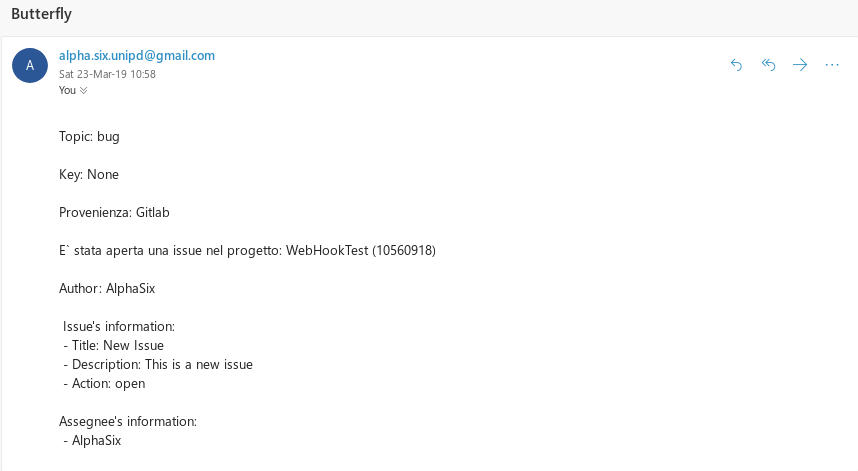
\includegraphics[width=\textwidth]{img/notifica_email_1.png}
	\caption{Formato dell' Email ricevuta da un utente finale}
\end{figure}

\subsubsection{Telegram}

Per ricevere le notifiche via Telegram, è necessario fare un passaggio addizionale: va fornita l'autorizzazione al bot per poter inviare messaggi agli utenti.
Il bot è raggiungibile al seguente link:
\begin{center}
    \url{http://t.me/ButterflyBot}
\end{center}

Dare il comando \texttt{/start} per dare l'autorizzazione di inoltro dei messaggi al bot.
È necessario inoltre aggiungere tramite l'interfaccia del Gestore Personale il proprio account Telegram.
In qualsiasi momento sarà possibile bloccare il bot in caso non si voglia più ricevere messaggi relativi a Butterfly su Telegram, tramite le funzionalità dell'applicazione.
\begin{figure}[H]
	\centering
	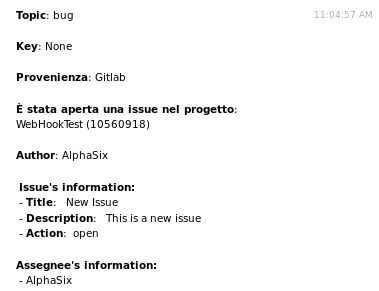
\includegraphics[width=10cm]{img/notifica_telegram_1.png}
	\caption{Formato del messaggio Telegram ricevuto da un utente finale}
\end{figure}
Nel caso in cui si volesse utilizzare un altro bot, i passaggi da seguire possono essere trovati sulla pagina apposita della documentazione di Telegram\footnote{\url{https://core.telegram.org/bots}}.
Per comunicare con questo bisogna modificare la variabile di ambiente \texttt{BUTTERFLY\_CONSUMER\_TELEGRAM\_BOT} che rappresenta il \texttt{token} univoco del nuovo bot, come descritto in \S\ref{var_consumer}.
